\documentclass{article}
\usepackage[a4paper,top=1.3cm,bottom=1cm,left=1.5cm,right=1.5cm,marginparwidth=0.75cm]{geometry}

\usepackage[14pt]{extsizes}
\usepackage{fancyhdr}
\usepackage{graphicx}
\usepackage[english,russian]{babel}
\usepackage{amsmath,amsfonts,amssymb,amsthm,mathtools}
\usepackage{physics}
\usepackage{wrapfig}
\usepackage{indentfirst}
\usepackage{gensymb}

\pagestyle{fancy}
\fancyfoot{}
\fancyfoot[R]{\thepage}
\fancyhead{}
\fancyhead[R]{Работа 1.4.1}

\begin{document}

\begin{titlepage}
	\vspace{5cm}
	{\huge
		\begin{center}
			{\bf Отчёт о выполнении лабораторной работы 1.4.1}\\
			Изучение физического маятника
		\end{center}
	}
	\vfill
	\begin{flushright}
		{\LARGE Подготовил\\ Лукин Иван \\
			\vspace{0.2cm}
			Б03-204}
	\end{flushright}
	\vspace{2cm}
	\begin{center}
		\today
	\end{center}
\end{titlepage}

\section*{}

\textbf{Цель работы:} исследовать зависимость периода колебаний физического маятника от его момента инерции. \\
\textbf{Оборудование:} физический маятник (однородный стальной стержень), опорная призма, математический маятник, счетчик числа колебаний, линейка, секундомер.

\section{Теоретическая часть}

\begin{wrapfigure}{l}{7cm}
	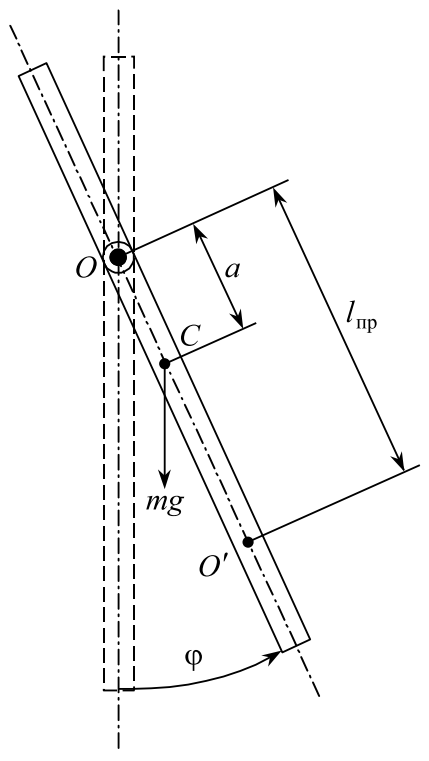
\includegraphics[width=1\linewidth]{ustanovka.png}
	\caption{Физический маятник}
\end{wrapfigure}

Физический маятник --- любое твёрдое тело, которое, находясь под действием силы тяжести, может свободно качаться вокруг неподвижной оси. Движение маятника можно описать следующим уравнением:

\begin{equation} \label{baza}
I\dv[2]{\varphi}{t}=M \text{,}
\end{equation}

где \(I\) --- момент инерции маятника, \(\varphi\) --- угол отклонения маятника от положения равновесия, \(M\) --- момент сил, действующих на маятник. \par
В данной работе в качестве физического маятника (рис. 1) используется однородный стальной стержень длиной \(l\); на нём закреплена опорная призма, которую можно перемещать вдоль стержня, меняяя расстояние \(OC\) от точки опоры маятника \(O\) до его центра масс \(C\). Если принять длину отрезка \(OC \text{ за } a \), то можно найти момент инерции маятника \(I\) по теореме Гюйгенца-Штейнера:
\[
I = \frac{ml^2}{12} + ma^2 \text{,} 
\]
где \(m\) - масса маятника. При малых углах отклонения \(\varphi\) момент силы тяжести, действующий на маятник, можно найти по следующей формуле:
\[
M = -mga\sin{\varphi} \approx -mga\varphi
\]

Мы не будем учитывать момент силы трения, так как он принебрежимо мал: в исправной установке маятник совершает несколько сот колебаний без заметного затухания. Подставляя полученные формулы для \(I\) и \(M\) в формулу (\ref{baza}), получим следующее выражение:

\begin{equation} \label{wave}
\ddot{\varphi} + \omega^2\varphi = 0 \text{,}
\end{equation}
где
\begin{equation} \label{omega}
\omega^2 = \frac{ag}{a^2+\frac{l^2}{12}} \text{.}
\end{equation} 
Из  (\ref{omega}) по известной формуле периода колебаний \(T = \dfrac{2\pi}{\omega}\) следует, что
\begin{equation} \label{period}
T = 2\pi\sqrt{\frac{a^2+\frac{l^2}{12}}{ag}}
\end{equation}
Видно, что период малых колебаний (при достаточно малом угле \(\varphi\)) не зависит ни от фазы, ни от амплитуды колебаний, так как, согласно формуле (\ref{omega}), \(\omega\) зависит лишь от \(g \text{, } l \text{ и } a\).\par
Проведя аналогию с математическим маятником, из формулы \(T' = 2\pi\sqrt{\dfrac{l'}{g}}\) получим следующую величину
\begin{equation} \label{lpr}
l_\text{пр} = a + \frac{l^2}{12a} \text{,}
\end{equation} 
которую называют приведённой длиной физического маятника. Поэтому точку $ O' $, отстоящую от точки опоры на расстояние $ l_\text{пр} $, называют центром качания физического маятника. Точка опоры и центр качания маятника обратимы, т.е. при качании маятника вокруг  точки $ O' $ период будет таким же, как и при качании вокруг точки $ O $.

\section{Практическая часть}

\subsection*{Определение диапазона амплитуд, при котором период колебаний не зависит от амплитуды}
Проведём измерения времени \(t\) 100 колебаний \(N\) физического маятника при разных углах отклонения \(\varphi\) для того, чтобы определить диапазанон амплитуд, в котором период колебаний не зависит от угла отклонения стержня \(\varphi\) от положения равновесия.  Результаты измерений занесем в таблицу \ref{tab1}.
\begin{table}[h!]
\centering
\begin{tabular}{|c|c|c|c|c|} \hline
	\(\varphi, \degree\) & \(t\), с & \(N\) & \(T\), с   & $ T_\text{ср} $, с \\ \hline
10  & 154,37                & 100                   & 1,5437                &                       \\
10  & 154,06                & 100                   & 1,5406                & 1,54203                 \\
10  & 154,18                & 100                   & 1,5418                &                       \\ \hline
5   & 153,91                & 100                   & 1,5391                &                       \\
5   & 153,97                & 100                   & 1,5397                & 1,53970                 \\
5   & 154,03                & 100                   & 1,5403                &             \\       
\hline    
\end{tabular} 
\caption{Результаты определения диапазона амплитуд}
\label{tab1}
\end{table}

Определим погрешность измерений с учётом того, что погрешность измерения секундомером равна \(\sigma_\text{с} = 0,2 \text{с}\).
\[
\sigma_\text{случ} = \sqrt{\frac{1}{N}\sum_{i=1}^{N}\left( T_\text{ср} - T_i \right)^2 },
\]
\[
\sigma_\text{сист} = \sigma_\text{с},
\]
\[
\sigma = \sqrt{\sigma_\text{с}^2+\sigma_\text{сл}^2}.
\]
По результатам вычислений мы определили для \(\varphi = 10\degree\) и \(\varphi = 5\degree\) \(T_\text{1} = 1.5 \pm 0.1 \text{ с}\) и \(T_\text{2} = 1.5 \pm 0.1 \text{ с}\), \(T_\text{1}\) и \(T_\text{2}\) совпадают в пределах погрешности. Значит, дальнейшие эксперименты можно проводить при \(\varphi \leq 10\degree\).
\subsection*{Вычисление ускорения свободного падения и длины стержня}
Перемещая опорную призму вдоль стержня, будем исследовать зависимость периода колебаний \(T\) от расстояния \(a\) между точкой опоры и центром масс. Сделав 10 измерений при \(N = 100\), занесём результаты в таблицу \ref{tab2}. 
\begin{table}[h!]
\centering
\begin{tabular}{|c|c|c|} \hline
\(a\), см & \(t\), с   & \(T\), с   \\ \hline
37    & 153,81 & 1,5381 \\
34    & 152,53 & 1,5253 \\
30    & 151,56 & 1,5156 \\
25    & 152,19 & 1,5219 \\
20    & 156,57 & 1,5657 \\
15    & 167,94 & 1,6794 \\
13    & 175,19 & 1,7519 \\
18    & 160,13 & 1,6013 \\
23    & 153,47 & 1,5347 \\
28    & 151,53 & 1,5153 \\
\hline
\end{tabular}
\caption{Зависимость периода колебаний от расстояния между точкой опоры и центра масс}
\label{tab2}
\end{table}
\noindent

Из формулы (\ref{period}) можно вывести линейную зависимость \(T^{2}a \text{ от } a^{2}\):
\begin{equation} \label{linear}
T^2a=\frac{4\pi^2}{g}a^2+\frac{\pi^2l^2}{3g}.
\end{equation}
\begin{table}[h!]
\centering
\begin{tabular}{|c|c|} \hline
\(a^2\), \(\text{см}^2\) & \(T^2a\), \(\text{с}^2\cdot\text{см}\) \\ \hline
1369      & 87,53281    \\
1156      & 79,10236     \\
900       & 68,91130     \\
625       & 57,90449     \\
400       & 49,02832      \\
225       & 42,30576      \\
169       & 39,89899     \\
324       & 46,15491     \\
529       & 54,17199     \\
784       & 64,29175     \\ 
\hline
\end{tabular}
\caption{Данные для графика}
\label{tab3}
\end{table}

По таблице \ref{tab3} построим график функции \(T^{2}a \text{ от } a^{2}\). При помощи МНК найдём коэффициенты
\begin{equation}
k=\dfrac{4\pi^2}{g}\text{ и } b =\dfrac{\pi^2l^2}{3g}.
\label{coefficients}
\end{equation}
Необходимые формулы: \\
Собственно коэффициенты
\[
k=\frac{\langle a^2\cdot T^2a\rangle-\langle a^2\rangle \langle T^2a\rangle}{\langle a^4\rangle - \langle a^2\rangle^2},
\]
\[
b=\langle T^2a \rangle -k\langle a^2 \rangle.
\]
Их случайные погрешности по МНК:
\[
\sigma_k^\text{случ}=\sqrt{\frac{1}{N}\left(\frac{\langle \left(T^2a\right) ^2 \rangle - \langle T^2a \rangle^2}{\langle a^4 \rangle - \langle a^2 \rangle^2} - k^2 \right) },
\]
\[
\sigma_b^\text{случ}= \sigma_k^\text{случ} \sqrt{\langle a^4 \rangle - \langle a^2  \rangle^2}.
\]
Систематические погрешности зависят от приборов, которыми мы пользовались для измерения величин:
\[
\sigma^\text{сист}_k = k\sqrt{\left(\frac{\Delta_{a}}{2a_\text{макс}} \right)^2 + \left(\frac{\Delta_{T^2a}}{2T^2a_{\text{макс}}} \right)^2 },
\]
\[
\sigma^\text{сист}_b = b\sqrt{\left(\frac{\Delta_{a}}{2a_\text{макс}} \right)^2 + \left(\frac{\Delta_{T^2a}}{2T^2a_{\text{макс}}} \right)^2 },
\]
где 
\[\Delta_{a} = 2\Delta_{l} = 0,2 \text{ см},\] 
\[\Delta_{T^2a} = 2\Delta_{l}  \Delta_{T} = 0,04 \text{ см}.\]
Полные погрешности коэффициентов:
\[
\sigma_k = \sqrt{\left( \sigma_k^\text{случ} \right)^2 + \left( \sigma_k^\text{сист} \right)^2 }
\]
\[
\sigma_b = \sqrt{\left( \sigma_b^\text{случ} \right)^2 + \left( \sigma_b^\text{сист} \right)^2 }.	
\]

В итоге \(k=0,0396\pm0,0001 \text{ }\frac{\text{с}^2}{\text{см}}\) и \(b=33,244\pm0,024 \text{ }\text{см}\cdot\text{с}^2\). Выразим из формул (\ref{coefficients}) \(g\) и \(l\):
\[
g = \frac{4\pi^2}{k},
\]
\[
l=\sqrt{\frac{3bg}{\pi^2}}.
\]
Их погрешности:
\[
\sigma_g = g\frac{\sigma_k}{k}
\]
\[
\sigma_l = l\sqrt{\left( \frac{\sigma_b}{b}\right)^2 + \left( \frac{\sigma_g}{g}\right)^2}
\]
Получим \underline{\(g=9,96\pm0,03 \text{ } \frac{\text{м}}{\text{с}^2}\)} и \underline{\(l=100,4\pm0,3 \text{ см}\)}. 
\subsection*{Проверка совпадения периода колебания физического маятника с математическим}
Подберём длину математического маятника для \(a = 20 \text{ см}\) так, чтобы периоды физического маятника и математического совпали. Остановимся на \(l_{\text{м}}=62 см\). Результаты измерения периодов для колебания на этих длинах занесём в таблицу \ref{tab4}. 
\begin{table}[h!]
\centering
\begin{tabular}{|c|c|}
\hline
Маятник        & \(T\), с      \\ \hline
Физический     & 1,5657 \\
Математический & 1,5749 \\ \hline
\end{tabular}
\label{tab4}
\caption{Периоды колебаний для физического и математического маятников}
\end{table}
Периоды из таблицы \ref{tab4} отличаются на \(\varepsilon = \dfrac{T_{\text{м}}-T_{\text{ф}}}{T_{\text{ф}}} \cdot 100\% \approx 0,58 \%\), что попадает в \[\varepsilon_{T_{\text{ф}}}=\dfrac{\Delta_{T}}{T_{\text{ф}}}\cdot 100\% \approx 12,70\%.\] Периоды математического и физического маятников совпали в пределах \(\varepsilon\), теперь можно сравнить \(l_{\text{пр}}\) , которую можно получить по формуле (\ref{lpr}), и \(l_{\text{м}}\), полученную экспериментально.
В результате расчётов по формуле (\ref{lpr}), используя \(l_{\text{лин}} = 100,1 \text{ см}\), величину, измеренную линейкой, получим \(l_{\text{пр}} \approx 61,75 \text{ см } \approx l_{\text{м}}\). Формула (\ref{lpr}) справедлива.
\subsection*{Проверка обратимости точки подвеса и центра качания}
Найдём расстояние от центра масс до центра качания \(a_1\) по следующей формуле, взяв \(a = 20 \text{ см}\):
\[
a_1= l_{\text{пр}} - a = \frac{l^2}{12a} \approx 41,75 \text{ см}
\]
В результате период колебаний \(T_1 = 1,5629 \text{ см} \approx T_2 = 1,5657 \text{ см}\), где \(T_2\) взяли из таблицы \ref{tab2}. Периоды совпали, следовательно, точка подвеса и центр качания обратимы.
\section{Выводы}
Полученная величина \(g=9,96\pm0,03 \text{ } \dfrac{\text{м}}{\text{с}^2}\) не совпала с теоретической, которая равна \(9,8154\) \(\dfrac{\text{м}}{\text{с}^2}\) для московской широты, в пределах погрешности, однако довольно близка к ней. Длина \(l=100,4\pm0,3 \text{ см}\) совпала с измеренной \(l_{\text{лин}} = 100,1 \pm 0,1 \text{ см}\) в пределах погрешности. Формула (\ref{lpr}) справедлива так же, как и утверждение об обратимости точки подвеса и центра качания.
\end{document}